\documentclass[11pt,reqno]{amsart}
\usepackage[margin=1.15in]{geometry}
\usepackage{amsmath,amssymb,amsthm,mathtools}
\usepackage{graphicx}
\usepackage{booktabs}
\usepackage[colorlinks=true,linkcolor=blue,citecolor=blue,urlcolor=blue]{hyperref}
\usepackage{microtype}

\theoremstyle{plain}
\newtheorem{theorem}{Theorem}
\newtheorem{proposition}[theorem]{Proposition}
\newtheorem{corollary}[theorem]{Corollary}
\newtheorem{lemma}[theorem]{Lemma}
\theoremstyle{definition}
\newtheorem{definition}[theorem]{Definition}
\newtheorem{remark}[theorem]{Remark}
\newtheorem{observation}[theorem]{Observation}

\DeclareMathOperator{\sqf}{sqf}
\newcommand{\Art}{\mathrm{A}}
\newcommand{\Leg}[2]{\left(\frac{#1}{#2}\right)}
\newcommand{\Z}{\mathbb{Z}}
\newcommand{\Q}{\mathbb{Q}}

\begin{document}

\title[Exclusion laws for consecutive Artin primes]
{Exclusion laws for consecutive Artin primes in arbitrary bases}

\author{Josh Bald}
\address{Ontario, Canada}
\email{jpbald93@gmail.com}

\subjclass[2020]{Primary 11A07; Secondary 11N05, 11N13, 11Y16, 11Y60}
\keywords{Artin's conjecture, primitive roots, consecutive primes, quadratic
characters, prime discriminants, Lemke Oliver--Soundararajan bias}

\date{\today}

\begin{abstract}
Say that a prime $p$ is \emph{Artin base $a$} if $a$ is a primitive root modulo
$p$. We prove that for every non-square base $a$ there is an explicit set of
gap classes at which two primes can \emph{never} both be Artin base $a$: if the
gap $g = q - p$ lies in one of these classes, the quadratic character
$\chi_a$ satisfies $\chi_a(q) = -\chi_a(p)$, so one of the two primes is a
quadratic residue base $a$ and hence not a primitive root. We classify these
\emph{exclusion classes} completely in terms of the factorization of the
discriminant of $\Q(\sqrt{a})$ into prime discriminants, and we deduce a clean
dichotomy: base $a$ admits an exclusion law if and only if the squarefree part
$d$ of $a$ satisfies $d \equiv 0 \pmod 2$, $d \equiv 3 \pmod 4$, or
$3 \mid d$. In particular bases with $d \equiv 1 \pmod 4$ odd and $3 \nmid d$
--- the smallest being $d = 5, 13, 17, 29$ --- admit \emph{no} exclusion law at
all. The classification is verified by exhaustive computation for all
non-square $2 \le a \le 30$, and the exclusion law itself is verified on
$63{,}105{,}745$ consecutive prime pairs below $10^9$ across seven bases, with
zero exceptions.

We then measure, for eleven bases, the consecutive-pair Artin correlation
$\delta(a)$ over all $50{,}847{,}531$ consecutive prime pairs below $10^9$.
Here the outcome is negative in an instructive way. One might expect bases with
denser exclusion classes to exhibit stronger anticorrelation; they do not. The
association with exclusion density is weak ($r = 0.23$), and base $5$, which
admits no exclusion law whatsoever, has the \emph{largest} $|\delta|$ of the
eleven. Instead $|\delta(a)|$ is governed by the size of the conductor $f$ of
$\chi_a$, with $r(\log f, |\delta|) = -0.96$. We conclude that the two
phenomena are genuinely distinct: the exclusion law is locally absolute but
globally negligible, while the global correlation is a conductor-size effect
inherited from the Lemke Oliver--Soundararajan bias.
\end{abstract}

\maketitle

\section{Introduction}
\label{sec:intro}

Artin's conjecture on primitive roots asserts that for a non-square integer
$a \neq -1$ the set of primes $p$ for which $a$ is a primitive root modulo $p$
has a positive density, given by an explicit rational multiple of Artin's
constant. It is known under GRH by Hooley~\cite{Hooley1967}, and
unconditionally for at least one of any three multiplicatively independent bases
by Gupta--Murty~\cite{GuptaMurty1984} and Heath-Brown~\cite{HeathBrown1986}; see
Moree's survey~\cite{Moree2012} for the extensive literature, and
\cite{FanPollack2025, PeruccaShparlinski2025} for recent uniform versions.

Write
\[
  \Art_a = \{\, p \text{ prime} : a \text{ is a primitive root mod } p \,\},
\]
and call $p \in \Art_a$ an \emph{Artin prime base $a$}. All results above
concern a \emph{single} prime at a time. The behaviour of Artin primes in
\emph{pairs} has been studied much less. Garcia, Kahoro and
Luca~\cite{GarciaKahoroLuca2019} (see also~\cite{GarciaLucaShiUdell2020})
investigated primitive-root bias for twin primes; Pollack~\cite{Pollack2014}
and Baker--Pollack~\cite{BakerPollack2016} showed, under GRH, that there are
infinitely many bounded-gap runs of primes sharing a primitive root.

The starting point of this paper is an elementary but apparently unrecorded
observation. Since a quadratic residue cannot generate the cyclic group
$(\Z/p\Z)^\times$ of even order $p - 1$, membership in $\Art_a$ forces
$\chi_a(p) = -1$, where $\chi_a$ is the quadratic character attached to
$\Q(\sqrt{a})$. Because $\chi_a$ is a character modulo the conductor $f$ of
that field, the value $\chi_a(p)$ depends only on $p \bmod f$. Consequently, if
a shift $g$ has the property that it \emph{reverses} $\chi_a$ on every
admissible residue class modulo $f$, then for any two primes $p$ and $q = p+g'$
with $g' \equiv g \pmod f$ we get $\chi_a(q) = -\chi_a(p)$, so at least one of
$\chi_a(p), \chi_a(q)$ equals $+1$ --- and that prime is not Artin base $a$.
Two primes at such a gap can never \emph{both} be Artin base $a$. We call this
an \emph{exclusion law} (Theorem~\ref{thm:exclusion}).

Our main theorem determines, for every base, exactly which gap classes are
exclusion classes.

\begin{theorem}[Classification; see Theorem~\ref{thm:classification}]
Let $a$ be a non-square positive integer with squarefree part $d$, let $D$ be
the discriminant of $\Q(\sqrt{d})$, and factor $D = D_1 D_2 \cdots D_k$ into
prime discriminants. Then an even shift $g$ is an exclusion class for base $a$
if and only if no component $D_i$ is \emph{indeterminate} at $g$ and an odd
number of the components \emph{reverse} at $g$, where the behaviour of each
component is given by Table~\ref{tab:components}.
\end{theorem}

The classification is sharp enough to answer the qualitative question
completely.

\begin{corollary}[Dichotomy; see Corollary~\ref{cor:dichotomy}]
Base $a$ admits at least one exclusion class if and only if $d$ is even, or
$d \equiv 3 \pmod 4$, or $3 \mid d$. Equivalently, if and only if the
prime-discriminant factorization of $D$ contains one of $-4$, $\pm 8$, $-3$.
\end{corollary}

Thus for $d \in \{5, 13, 17, 29, 37, 41, 53, 61, \dots\}$ there is no exclusion
law at all, while for $d = 3$ (and $d = 12, 27, \dots$) fully half of the even
gap classes modulo $12$ are exclusion classes. This is a genuine structural
dichotomy, not an artifact of small conductors, and its source is a
degeneration of a Jacobi-sum obstruction at the single prime $3$
(Remark~\ref{rem:three}).

In the second half of the paper we turn from the deterministic statement to a
statistical one. For a base $a$ define the consecutive-pair correlation
\begin{equation}
\label{eq:delta}
  \delta(a) \;=\; P\bigl(p_{n+1} \in \Art_a \mid p_n \in \Art_a\bigr)
             \;-\; P\bigl(p_{n+1} \in \Art_a \mid p_n \notin \Art_a\bigr),
\end{equation}
estimated over consecutive primes $p_n < p_{n+1} \le x$. The bias of
Lemke Oliver and Soundararajan~\cite{LOS2016} in the joint distribution of
$(p_n \bmod m, p_{n+1} \bmod m)$ propagates, through the factorization of
$p - 1$, into Artin status, so one expects $\delta(a) \neq 0$; and indeed we
find $\delta(a) < 0$ for all eleven bases examined, with $|z| \ge 96$
throughout.

The natural guess is that the exclusion law drives this anticorrelation: bases
whose exclusion classes capture a larger share of consecutive pairs should
display a more negative $\delta$. \emph{This guess is false}, and we regard its
refutation as one of the contributions of this paper. Over all
$50{,}847{,}531$ consecutive prime pairs below $10^9$ we find

\begin{itemize}
\item base $5$, which admits \emph{no} exclusion law, has the largest
      $|\delta|$ of the eleven bases;
\item base $3$, whose exclusion classes capture $53\%$ of all consecutive pairs
      by weight, ranks only third;
\item the mean $|\delta|$ over bases \emph{with} an exclusion law is $0.0296$,
      versus $0.0411$ over bases \emph{without} one --- a ratio of $0.72$, in
      the direction opposite to the guess;
\item $r(\text{exclusion weight}, |\delta|) = 0.23$, whereas
      $r(\log f, |\delta|) = -0.96$.
\end{itemize}

The explanation is a matter of scale rather than of mechanism. An exclusion
class imposes an absolute constraint, but only on a restricted set of gap
classes; averaged over all pairs, the constraint is diluted. What survives in
the average is the number of residue channels available to $\chi_a$, which is
controlled by $f$: the smaller the conductor, the fewer the classes over which
the Lemke Oliver--Soundararajan transition bias is distributed, and the larger
the resulting per-base correlation. We state this as a measured empirical law
(Observation~\ref{obs:conductor}) rather than a conjectured exact power of $f$,
because the data do not support a clean exponent.

\subsection*{Summary of results}
Section~\ref{sec:exclusion} proves the exclusion law and the classification and
establishes the dichotomy. Section~\ref{sec:computation} describes the
computation. Section~\ref{sec:verification} reports the verification of the
exclusion law at $10^9$. Section~\ref{sec:delta} reports the measurement of
$\delta(a)$, the refutation of the exclusion-density hypothesis, and the
conductor law. Section~\ref{sec:discussion} discusses what we take the
consequences to be.

\section{The exclusion law and its classification}
\label{sec:exclusion}

Throughout, $a \ge 2$ is an integer that is not a perfect square, $d = \sqf(a)$
denotes its squarefree part, and
\begin{equation}
\label{eq:disc}
  D = \begin{cases} d, & d \equiv 1 \pmod 4,\\ 4d, & \text{otherwise,}\end{cases}
  \qquad f = |D|,
\end{equation}
so that $D$ is the discriminant of $K = \Q(\sqrt{a}) = \Q(\sqrt{d})$ and $f$ is
the conductor of the associated quadratic character
$\chi_a = \Leg{d}{\cdot}$. By quadratic reciprocity $\chi_a$ is a Dirichlet
character modulo $f$; in particular
\begin{equation}
\label{eq:modf}
  \chi_a(p) \text{ depends only on } p \bmod f \qquad (p \nmid 2d).
\end{equation}

We recall the elementary obstruction, which is the only number-theoretic input
to Theorem~\ref{thm:exclusion}.

\begin{lemma}
\label{lem:obstruction}
Let $p > 2$ be a prime with $p \nmid a$. If $a$ is a primitive root modulo $p$
then $\chi_a(p) = -1$.
\end{lemma}

\begin{proof}
If $\chi_a(p) = +1$ then $a \equiv b^2 \pmod p$ for some $b$, whence
$a^{(p-1)/2} \equiv b^{p-1} \equiv 1 \pmod p$. Since $p > 2$, $(p-1)/2 < p-1$,
so the multiplicative order of $a$ is a proper divisor of $p - 1$ and $a$ is not
a primitive root.
\end{proof}

\begin{definition}
\label{def:shift}
Let $R_f \subseteq (\Z/f\Z)^\times$ be the set of residues attained by primes
$p \nmid 2d$. For an even integer $g$, say that $g$ is
\begin{itemize}
\item \emph{reversing} for $a$ if $\chi_a(r+g) = -\chi_a(r)$ for all $r \in R_f$
      with $r + g \in R_f$;
\item \emph{preserving} for $a$ if $\chi_a(r+g) = +\chi_a(r)$ for all such $r$;
\item \emph{indeterminate} otherwise.
\end{itemize}
A reversing class $g \bmod f$ is called an \emph{exclusion class} for base $a$.
\end{definition}

\begin{theorem}[Exclusion law]
\label{thm:exclusion}
Let $g$ be reversing for $a$. Then there is no pair of primes $p, q > 2$ with
$p, q \nmid a$, $q - p \equiv g \pmod f$, such that $a$ is a primitive root
modulo both $p$ and $q$.
\end{theorem}

\begin{proof}
By~\eqref{eq:modf} and Definition~\ref{def:shift},
$\chi_a(q) = \chi_a(p + (q-p)) = -\chi_a(p)$. Hence exactly one of
$\chi_a(p), \chi_a(q)$ equals $+1$, and by Lemma~\ref{lem:obstruction} the
corresponding prime is not Artin base $a$.
\end{proof}

Theorem~\ref{thm:exclusion} is unconditional and its proof is three lines; the
content lies in determining the reversing classes, which we now do. Recall that
every discriminant $D$ factors uniquely as a product of \emph{prime
discriminants}
\begin{equation}
\label{eq:primedisc}
  D = D_1 D_2 \cdots D_k, \qquad
  D_i \in \{-4\} \cup \{8, -8\} \cup \{\, q^* : q \text{ odd prime} \,\},
\end{equation}
where $q^* = q$ if $q \equiv 1 \pmod 4$ and $q^* = -q$ if $q \equiv 3 \pmod 4$;
the odd $D_i$ are precisely the $q^*$ for the odd primes $q \mid d$, and a
factor $\pm 4, \pm 8$ occurs according to $d \bmod 8$. Correspondingly
$\chi_a = \prod_i \chi_{D_i}$, with $\chi_{D_i}$ of conductor $|D_i|$.

\begin{table}[t]
\centering
\caption{Behaviour of each prime-discriminant component of $\chi_a$ under the
shift $r \mapsto r + g$. Here $q \ge 5$ is an odd prime.}
\label{tab:components}
\begin{tabular}{llll}
\toprule
component $D_i$ & conductor & reversing iff & preserving iff \\
\midrule
$-4$        & $4$ & $g \equiv 2 \pmod 4$   & $g \equiv 0 \pmod 4$ \\
$8$ or $-8$ & $8$ & $g \equiv 4 \pmod 8$   & $g \equiv 0 \pmod 8$ \\
$-3$        & $3$ & $g \not\equiv 0 \pmod 3$ & $g \equiv 0 \pmod 3$ \\
$q^*$, $q \ge 5$ & $q$ & never             & $g \equiv 0 \pmod q$ \\
\bottomrule
\end{tabular}
\end{table}

\begin{proposition}
\label{prop:components}
Table~\ref{tab:components} is correct: each component behaves as stated, and in
the cases not listed as reversing or preserving it is indeterminate. In
particular a component of conductor $8$ is indeterminate for
$g \equiv 2, 6 \pmod 8$, and a component $q^*$ with $q \ge 5$ is indeterminate
for every $g \not\equiv 0 \pmod q$.
\end{proposition}

\begin{proof}
\emph{Conductor $4$.} $\chi_{-4}(r) = (-1)^{(r-1)/2}$ depends only on
$r \bmod 4$, and on $\{1,3\}$ it is injective. A shift by $g \equiv 2 \pmod 4$
interchanges $1$ and $3$, hence reverses; $g \equiv 0 \pmod 4$ fixes both.

\emph{Conductor $8$.} $\chi_8(r) = +1$ iff $r \equiv \pm 1 \pmod 8$, so the
fibres are $\{1,7\}$ and $\{3,5\}$; the map $r \mapsto r + 4$ interchanges these
two sets, hence reverses, while $r \mapsto r$ preserves. For $g \equiv 2
\pmod 8$ we have $1 \mapsto 3$ (a reversal) but $3 \mapsto 5$ (a preservation),
so the behaviour depends on the class and $g$ is indeterminate; similarly for
$g \equiv 6$. The same computation applies to $\chi_{-8}$, whose $+1$-fibre is
$\{1,3\}$ and whose $-1$-fibre is $\{5,7\}$, again interchanged by $+4$.

\emph{Conductor $3$.} $\chi_{-3}(r) = +1$ iff $r \equiv 1 \pmod 3$. On the two
admissible classes $\{1,2\}$ the character is injective, so any
$g \not\equiv 0 \pmod 3$ moves $1 \leftrightarrow 2$ and reverses, while
$g \equiv 0$ preserves.

\emph{Conductor $q \ge 5$.} Suppose, for a contradiction, that
$\chi_{q^*}(r+g) = \varepsilon\, \chi_{q^*}(r)$ for a fixed $\varepsilon \in
\{\pm 1\}$, all $r$ with $r, r+g \not\equiv 0 \pmod q$, and some
$g \not\equiv 0 \pmod q$. Multiplying by $\chi_{q^*}(r)$ and summing over
$r \bmod q$ gives
\begin{equation}
\label{eq:jacobi}
  S(g) \;:=\; \sum_{r \bmod q} \chi_{q^*}(r)\,\chi_{q^*}(r+g)
        \;=\; \varepsilon \cdot \#\{\, r : r, r+g \not\equiv 0 \,\}
        \;=\; \varepsilon\,(q-2).
\end{equation}
On the other hand, for $g \not\equiv 0 \pmod q$ the substitution
$r = g t$ (legitimate since $g$ is invertible) and the complete
multiplicativity of $\chi_{q^*}$ give
\[
  S(g) = \sum_{t \bmod q} \chi_{q^*}(gt)\chi_{q^*}(g(t+1))
       = \chi_{q^*}(g)^2 \sum_{t} \chi_{q^*}(t)\chi_{q^*}(t+1)
       = \sum_{t \bmod q} \chi_{q^*}\!\left(\frac{t+1}{t}\right),
\]
the last sum being over $t \not\equiv 0$. As $t$ runs over the nonzero classes,
$u = (t+1)/t = 1 + t^{-1}$ runs over all classes except $u = 1$, whence
\[
  S(g) = \sum_{u \neq 1} \chi_{q^*}(u) = \left(\sum_{u \bmod q} \chi_{q^*}(u)\right) - \chi_{q^*}(1) = 0 - 1 = -1 .
\]
Comparing with~\eqref{eq:jacobi} forces $|{-1}| = q - 2$, i.e.\ $q = 3$. For
$q \ge 5$ this is a contradiction, so no such $\varepsilon$ exists and $g$ is
indeterminate. Finally $g \equiv 0 \pmod q$ clearly preserves.
\end{proof}

\begin{remark}
\label{rem:three}
The proof isolates precisely why the prime $3$ behaves differently from all
larger primes, and it is worth emphasising that this is structural rather than
an artifact. The Jacobi-type sum $S(g)$ equals $-1$ for \emph{every} $q$ and
every $g \not\equiv 0$, including $q = 3$; what fails at $q = 3$ is the
\emph{counting} side of~\eqref{eq:jacobi}, since $q - 2 = 1$ and
$\varepsilon(q-2) = \pm 1$ is then compatible with $S(g) = -1$. Concretely,
only one residue class survives the requirement that $r$ and $r+g$ both be
prime to $3$, and a sign condition imposed on a single class is vacuously
uniform. Thus the reversing behaviour of the component $-3$ --- which is what
makes base $3$ the most heavily constrained base --- sits exactly at the
boundary where the obstruction of Proposition~\ref{prop:components}
degenerates.
\end{remark}

\begin{theorem}[Classification of exclusion classes]
\label{thm:classification}
Let $a$ be non-square with $D = D_1 \cdots D_k$ as in~\eqref{eq:primedisc}, and
let $g$ be even. Then $g$ is reversing for $a$ if and only if no $D_i$ is
indeterminate at $g$ and the number of $i$ with $D_i$ reversing at $g$ is odd;
and $g$ is preserving if and only if no $D_i$ is indeterminate at $g$ and that
number is even.
\end{theorem}

\begin{proof}
Since $\chi_a = \prod_i \chi_{D_i}$ and the moduli $|D_i|$ are pairwise
coprime, the Chinese Remainder Theorem identifies $R_f$ with the product of the
component residue sets. If every component is reversing or preserving at $g$,
then for every $r$,
$\chi_a(r+g) = \prod_i \chi_{D_i}(r+g) = \bigl(\prod_i \varepsilon_i\bigr)\chi_a(r)$
where $\varepsilon_i = -1$ exactly for the reversing components; so $\chi_a$ is
reversed iff the count of such $i$ is odd. Conversely, suppose some component
$D_j$ is indeterminate at $g$, so there are $r_j, r_j'$ in its residue set with
$\chi_{D_j}(r_j + g) = -\chi_{D_j}(r_j)$ and
$\chi_{D_j}(r_j' + g) = +\chi_{D_j}(r_j')$. Fixing any admissible choices at
the other components and varying only the $j$-th coordinate via CRT produces
two residues $r, r' \in R_f$ at which $\chi_a$ is respectively reversed and
preserved. Hence $g$ is neither reversing nor preserving.
\end{proof}

\begin{corollary}[Dichotomy]
\label{cor:dichotomy}
Base $a$ admits at least one exclusion class if and only if
\[
  d \equiv 0 \!\!\pmod 2, \qquad\text{or}\qquad d \equiv 3 \!\!\pmod 4,
  \qquad\text{or}\qquad 3 \mid d,
\]
equivalently if and only if $\{-4, 8, -8, -3\} \cap \{D_1, \dots, D_k\} \neq
\emptyset$.
\end{corollary}

\begin{proof}
By Theorem~\ref{thm:classification} a reversing $g$ requires at least one
component that is reversing at $g$, and by Table~\ref{tab:components} the only
components capable of reversing are $-4$, $\pm 8$ and $-3$. The component $-4$
occurs iff $d \equiv 3 \pmod 4$, a component $\pm 8$ occurs iff $d$ is even,
and $-3$ occurs iff $3 \mid d$; this gives the stated equivalence of
conditions. Conversely, if such a component $D_j$ exists, choose $g$ by CRT to
lie in a reversing class of $D_j$ and in the class $0$ modulo $|D_i|$ for every
$i \neq j$, which is possible as the moduli are coprime; then every other
component preserves, exactly one reverses, and $g$ may be taken even (if
necessary replace $g$ by $g + f$, noting $f$ is even unless $f = d \equiv 1
\pmod 4$ is odd, in which case no reversing component exists and the case does
not arise). By Theorem~\ref{thm:classification}, $g$ is reversing.
\end{proof}

\begin{remark}
The smallest bases with no exclusion law are therefore those with
$d \in \{5, 13, 17, 29, 37, 41, 53, 61, \dots\}$, i.e.\ $d \equiv 1 \pmod 4$,
$d$ odd, $3 \nmid d$. Among $2 \le a \le 30$ these are $a = 5, 13, 17, 20, 29$
(note $\sqf(20) = 5$). At the other extreme, $d \equiv 3 \pmod{4}$ with
$3 \mid d$ gives $f = 12$ and \emph{three} of the six even classes modulo $12$
are exclusion classes; this occurs for $a = 3, 12, 27, \dots$.
\end{remark}

\subsection*{Computational confirmation of the classification}
For each non-square $a$ with $2 \le a \le 30$ we computed the reversing and
preserving sets directly, by evaluating $\chi_a$ on every residue class in
$R_f$ attained by a prime below $2 \times 10^5$ and testing
Definition~\ref{def:shift} exhaustively over all even $g$ modulo $f$. The
resulting sets agree \emph{exactly}, in every case, with the prediction of
Theorem~\ref{thm:classification}; and the criterion of
Corollary~\ref{cor:dichotomy} was confirmed for all non-square $2 \le a \le 79$.
Table~\ref{tab:classification} records a representative sample.

\begin{table}[t]
\centering
\caption{Exclusion classes for selected bases. ``Prime discs.'' lists the
factorization~\eqref{eq:primedisc}; the exclusion classes are those predicted by
Theorem~\ref{thm:classification} and confirmed by exhaustive search.}
\label{tab:classification}
\begin{tabular}{rrlll}
\toprule
$a$ & $f$ & prime discs. & exclusion classes mod $f$ & preserving classes \\
\midrule
$2$  & $8$   & $8$          & $4$          & $0$ \\
$3$  & $12$  & $-3, -4$     & $4, 6, 8$    & $0, 2, 10$ \\
$5$  & $5$   & $5$          & \emph{none}  & \emph{none} \\
$6$  & $24$  & $-3, -8$     & $8, 12, 16$  & $0, 4, 20$ \\
$7$  & $28$  & $-7, -4$     & $14$         & $0$ \\
$10$ & $40$  & $5, 8$       & $20$         & $0$ \\
$11$ & $44$  & $-11, -4$    & $22$         & $0$ \\
$13$ & $13$  & $13$         & \emph{none}  & \emph{none} \\
$15$ & $60$  & $-3, 5, -4$  & $20, 30, 40$ & $0, 10, 50$ \\
$17$ & $17$  & $17$         & \emph{none}  & \emph{none} \\
$21$ & $21$  & $-3, -7$     & $14$         & \emph{none} \\
$29$ & $29$  & $29$         & \emph{none}  & \emph{none} \\
$30$ & $120$ & $-3, 5, -8$  & $40, 60, 80$ & $0, 20, 100$ \\
\bottomrule
\end{tabular}
\end{table}

\section{Data and computation}
\label{sec:computation}

We enumerated the primes up to $x = 10^9$ by a segmented sieve of Eratosthenes
with segment length $2^{22}$, obtaining $50{,}847{,}532$ primes $p \ge 5$ and
hence $50{,}847{,}531$ consecutive pairs. For each prime $p$ we factored
$p - 1$ once, by trial division over the primes below $10^5$ together with the
cofactor, and then tested primitive-root status for all of the bases
\[
  a \in \{2, 3, 5, 6, 7, 10, 11, 13, 17, 21, 29\}
\]
simultaneously, using the standard criterion that $a$ is a primitive root
modulo $p$ iff $a^{(p-1)/\ell} \not\equiv 1 \pmod p$ for every prime
$\ell \mid p-1$. Modular exponentiation was carried out in $128$-bit arithmetic.
Sharing the factorization of $p-1$ across all eleven bases is what makes the
computation inexpensive; the entire run takes under an hour on a single core and
writes no intermediate table, accumulating instead the $2\times 2$ contingency
counts of (Artin status of $p_n$, Artin status of $p_{n+1}$), both globally and
separately for each gap $g \le 300$.

The base set was chosen to span the dichotomy of
Corollary~\ref{cor:dichotomy}: $a = 5, 13, 17, 29$ admit no exclusion law,
$a = 3$ and $a = 6$ have three exclusion classes each, and
$a = 2, 7, 10, 11, 21$ have one. All counts reported below are exact; no
sampling is involved. The implementation, together with an independent and
slower verification in \texttt{sympy} used to cross-check the exclusion counts
at $3 \times 10^6$, is available at the repository cited in the data
availability statement.

\section{Verification of the exclusion law at \texorpdfstring{$10^9$}{10^9}}
\label{sec:verification}

Theorem~\ref{thm:exclusion} is a proved statement, so a computation cannot
strengthen it; but it is a sharp and easily falsified prediction about a large
finite set, and checking it guards against errors in the classification of
Theorem~\ref{thm:classification} and in the implementation. For each base with
at least one exclusion class we counted the consecutive prime pairs
$(p_n, p_{n+1})$ whose gap lies in an exclusion class, and among those the pairs
that are doubly Artin. Table~\ref{tab:verification} reports the result.

\begin{table}[t]
\centering
\caption{Exclusion law at $x = 10^9$. ``Pairs'' counts consecutive prime pairs
whose gap lies in an exclusion class for the given base; ``both Artin'' counts
those in which $a$ is a primitive root modulo both primes. The control column
gives, for comparison, the proportion of doubly-Artin pairs at the preserving
class $g \equiv 0$.}
\label{tab:verification}
\begin{tabular}{rrlrrc}
\toprule
$a$ & $f$ & exclusion classes & pairs & both Artin & control (preserving) \\
\midrule
$2$  & $8$  & $4$         & $13{,}404{,}106$ & $0$ & $27.5\%$ \\
$3$  & $12$ & $4, 6, 8$   & $27{,}010{,}759$ & $0$ & $27.5\%$ \\
$6$  & $24$ & $8, 12, 16$ & $12{,}419{,}039$ & $0$ & $27.8\%$ \\
$7$  & $28$ & $14$        & $3{,}567{,}335$  & $0$ & $26.3\%$ \\
$10$ & $40$ & $20$        & $2{,}214{,}511$  & $0$ & $26.7\%$ \\
$11$ & $44$ & $22$        & $1{,}796{,}191$  & $0$ & $27.5\%$ \\
$21$ & $21$ & $14$        & $2{,}693{,}804$  & $0$ & --- \\
\midrule
\multicolumn{3}{l}{\emph{total}} & $63{,}105{,}745$ & $\mathbf{0}$ & \\
\bottomrule
\end{tabular}
\end{table}

There are $63{,}105{,}745$ pairs in exclusion classes and not a single
doubly-Artin pair among them, while at preserving classes the doubly-Artin
proportion lies between $26.3\%$ and $29.3\%$ throughout, as one expects from the square of
the relevant Artin density. (Base $21$ has no preserving class, by
Table~\ref{tab:classification}.) A supplementary check reproduced the
same zero counts, independently, with \texttt{sympy} order computations for
primes below $3 \times 10^6$.

\section{The consecutive-pair correlation across bases}
\label{sec:delta}

We now measure $\delta(a)$ of~\eqref{eq:delta}. Write $n_{ij}$ for the number
of consecutive pairs with Artin status $i$ at $p_n$ and $j$ at $p_{n+1}$, so
that
\[
  \widehat{\delta}(a) = \frac{n_{11}}{n_{10}+n_{11}} - \frac{n_{01}}{n_{00}+n_{01}},
\]
with the standard binomial standard error for a difference of two independent
proportions. Table~\ref{tab:delta} collects the results.

\begin{table}[t]
\centering
\caption{Consecutive-pair Artin correlation at $x = 10^9$, over all
$50{,}847{,}531$ consecutive prime pairs, sorted by $|\delta|$. Here
$\#\mathrm{exc}$ is the number of exclusion classes and $w$ the fraction of all
consecutive pairs whose gap lies in one.}
\label{tab:delta}
\begin{tabular}{rrrrrr}
\toprule
$a$ & $f$ & $\#\mathrm{exc}$ & $w$ & $\widehat{\delta}(a)$ & $z$ \\
\midrule
$5$  & $5$  & $0$ & $0.0000$ & $-0.066563$ & $-478.9$ \\
$2$  & $8$  & $1$ & $0.2636$ & $-0.050199$ & $-361.0$ \\
$3$  & $12$ & $3$ & $0.5312$ & $-0.046676$ & $-335.4$ \\
$13$ & $13$ & $0$ & $0.0000$ & $-0.042573$ & $-305.6$ \\
$21$ & $21$ & $1$ & $0.0530$ & $-0.038345$ & $-275.2$ \\
$17$ & $17$ & $0$ & $0.0000$ & $-0.033025$ & $-236.7$ \\
$6$  & $24$ & $3$ & $0.2442$ & $-0.025205$ & $-180.4$ \\
$29$ & $29$ & $0$ & $0.0000$ & $-0.022422$ & $-160.4$ \\
$11$ & $44$ & $1$ & $0.0353$ & $-0.018909$ & $-135.2$ \\
$10$ & $40$ & $1$ & $0.0436$ & $-0.014140$ & $-101.0$ \\
$7$  & $28$ & $1$ & $0.0702$ & $-0.013491$ & $-96.4$ \\
\bottomrule
\end{tabular}
\end{table}

Two features stand out. First, $\delta(a) < 0$ for every base, with $|z| \ge
96$: consecutive primes \emph{repel} in Artin status, uniformly in the base.
This is consistent with the mechanism proposed for the base-$10$ case, namely
that the Lemke Oliver--Soundararajan bias~\cite{LOS2016} in the joint
distribution of consecutive prime residues propagates through the factorization
of $p-1$ --- and hence through $\omega(p-1)$, whose consecutive values are
themselves anticorrelated --- into Artin status.

Second, and contrary to what the first half of this paper might suggest, the
ordering of $|\delta(a)|$ has almost nothing to do with the exclusion law.

\begin{observation}[Refutation of the exclusion-density hypothesis]
\label{obs:refutation}
The hypothesis that $|\delta(a)|$ increases with the density $w$ of exclusion
classes is false. At $x = 10^9$:
\begin{enumerate}
\item base $5$, for which Corollary~\ref{cor:dichotomy} shows no exclusion class
      exists, has the largest $|\delta|$ among the eleven bases;
\item base $3$, whose exclusion classes contain $53\%$ of all consecutive pairs,
      ranks third;
\item the mean of $|\delta|$ over the seven bases with an exclusion law is
      $0.0296$, against $0.0411$ over the four without, a ratio of $0.72$ ---
      opposite in direction to the hypothesis;
\item $r(w, |\delta|) = 0.23$ over the eleven bases, and the apparent weak
      positive association is confounded, since small conductors are exactly the
      even and $3$-divisible ones.
\end{enumerate}
\end{observation}

The reason is one of scale rather than of mechanism, and in hindsight it is
clear. An exclusion class is an absolute prohibition, but it applies only to
certain gap classes; the statistic $\delta(a)$ averages over all consecutive
pairs, in which those classes are a minority, so the prohibition is diluted.
Indeed the exclusion classes contribute to $\delta$ only through the pairs they
contain, and their effect is bounded by $w$ times a quantity of order the Artin
density --- for base $10$, where $w = 0.044$, this bound is already smaller than
the observed $|\delta|$.

What does organise the data is the conductor.

\begin{observation}[Conductor law]
\label{obs:conductor}
Over the eleven bases at $x = 10^9$,
\[
  r(\log f, |\delta|) = -0.957, \qquad
  r(f^{-1/2}, |\delta|) = +0.951, \qquad
  r(f^{-1}, |\delta|) = +0.921,
\]
against $r(w, |\delta|) = +0.231$ for the exclusion density. Thus
$|\delta(a)|$ is a decreasing function of the conductor of $\chi_a$, and this
single parameter accounts for the observed ordering far better than any
exclusion-based quantity.
\end{observation}

The heuristic is that $\chi_a$ is determined modulo $f$, so the residue
information relevant to Artin status base $a$ is carried by the
$\varphi(f)$ classes in $(\Z/f\Z)^\times$. The transition bias
of~\cite{LOS2016} is distributed across these channels; the fewer the channels,
the less the cancellation between them, and the larger the surviving global
correlation. Figure~\ref{fig:conductor} displays both associations.

\begin{figure}[t]
\centering
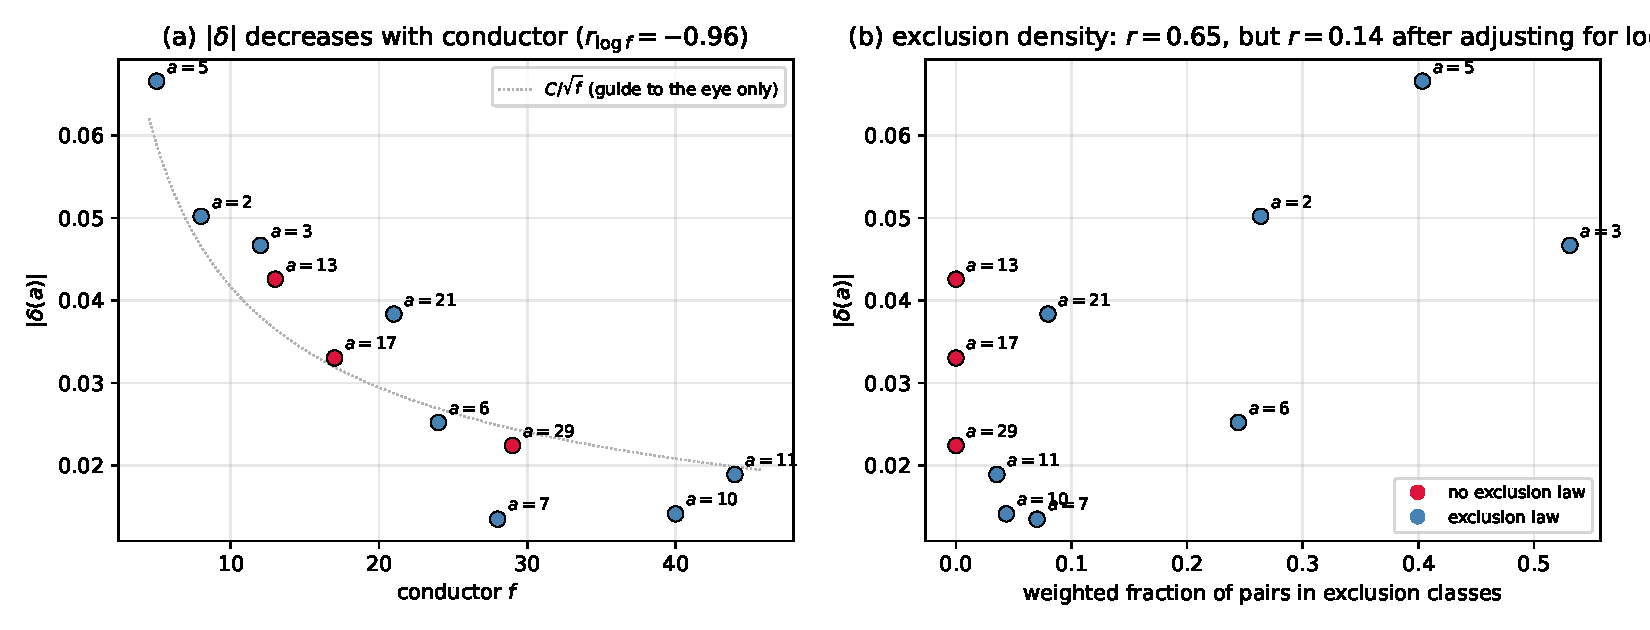
\includegraphics[width=\textwidth]{fig_delta_conductor.pdf}
\caption{Left: $|\delta(a)|$ against the conductor $f$ of $\chi_a$ at
$x = 10^9$. The data points are the content of the figure; the faint dotted
curve $C/\sqrt{f}$ ($C = 0.132$) is a guide to the eye only --- as discussed
after Observation~\ref{obs:conductor}, the data do not identify an exponent and
no power law is asserted. Right: $|\delta(a)|$ against the weighted fraction of
consecutive pairs lying in exclusion classes. Bases admitting no exclusion law
are shown in red; one of them has the largest $|\delta|$ of all.}
\label{fig:conductor}
\end{figure}

We deliberately refrain from asserting an exact power law. The products
$|\delta| \cdot f$ drift from $0.33$ to $0.83$ across the range, while
$|\delta| \cdot \sqrt{f}$ drift only from $0.15$ to $0.13$; so $f^{-1/2}$ is the
better one-parameter description, but neither is constant, and with eleven bases
spanning $5 \le f \le 44$ we regard the evidence as insufficient to identify an
exponent. The honest statement is Observation~\ref{obs:conductor}: a strong
monotone dependence on $f$, whose precise shape should be derived from, rather
than fitted ahead of, a channel-by-channel analysis.

\begin{remark}
The two smallest $|\delta|$ belong to $a = 7$ and $a = 10$, with $f = 28$ and
$f = 40$; the largest to $a = 5$ with $f = 5$. Note that $a = 21$, with
$f = 21$, sits above both $a = 17$ ($f = 17$) and $a = 6$ ($f = 24$), so the
dependence on $f$ is not perfectly monotone --- as one would expect if the
relevant quantity is a sum over the $\varphi(f)$ channels rather than a function
of $f$ alone.
\end{remark}

\section{Discussion}
\label{sec:discussion}

\subsection*{What is new here}
The ingredients are classical: the quadratic obstruction to being a primitive
root, quadratic reciprocity, the decomposition of a discriminant into prime
discriminants, and the elementary evaluation of a Jacobi-type character sum. The
contributions are (i) the observation that these combine into a
\emph{deterministic exclusion law} for consecutive Artin primes, valid in every
base (Theorem~\ref{thm:exclusion}); (ii) a \emph{complete classification} of
the exclusion classes in terms of prime discriminants
(Theorem~\ref{thm:classification}), with the resulting dichotomy
(Corollary~\ref{cor:dichotomy}) identifying exactly which bases admit no such
law; and (iii) the first cross-base measurement of the consecutive-pair Artin
correlation, which refutes the natural hypothesis that the exclusion law drives
that correlation and identifies conductor size as the operative parameter
instead.

We regard (iii) as no less useful than (i) and (ii). The exclusion law is
visually striking --- tens of millions of pairs with an exact zero count --- and
it would be easy to assume that it dominates the statistics of Artin primes in
pairs. It does not. Separating a locally absolute but globally negligible
constraint from the globally operative conductor effect seems to us the right
conclusion to draw, and it is one we reached only by measuring.

\subsection*{Relation to earlier work}
For base $10$ the exclusion class $g \equiv 20 \pmod{40}$ and a measurement of
$\delta(10)$ were obtained by the author in earlier work; the present paper
subsumes that case, since $d = 10$ gives $D = 40 = 5 \cdot 8$ and
Theorem~\ref{thm:classification} returns the single exclusion class
$g \equiv 20$. Garcia--Kahoro--Luca~\cite{GarciaKahoroLuca2019} study
primitive-root bias for twin primes, i.e.\ the single gap $g = 2$; our
Table~\ref{tab:components} shows that $g = 2$ is an exclusion class exactly when
some reversing component has $g = 2$ in its reversing class and no component is
indeterminate there, which for $g = 2$ requires $f \mid 12$ --- so
$a \equiv 3, 12, 27, \dots$ are the twin-prime cases covered by our law.
Pollack~\cite{Pollack2014} and Baker--Pollack~\cite{BakerPollack2016}
construct, under GRH, bounded-gap runs of primes sharing a primitive root; our
results add a base-specific constraint on where such runs can occur, since a run
in base $a$ must avoid every exclusion class of $a$, and for $a = 3$ this
excludes half of the available even gaps.

\subsection*{Future work}
Three directions suggest themselves. First, the channel decomposition displayed
after Observation~\ref{obs:conductor} should be carried out: a derivation from
the singular series of~\cite{HardyLittlewood1923} together with Hooley's
density computation~\cite{Hooley1967}, summed over the $\varphi(f)$ residue
channels, would replace an empirical regularity with a formula and settle the
exponent question. Second, the decay of $\delta(a)$ in $x$ should be measured for several
bases at once; for base $10$ a decay of order $1/\log x$ was conjectured, and
the present pipeline extends to $10^{12}$ without difficulty. Third, the
classification invites an analogue for higher-order obstructions: membership in
$\Art_a$ also requires $a$ to be a non-$\ell$-th-power residue for every
$\ell \mid p-1$, and the cubic case in particular should produce exclusion laws
governed by conductors of cubic characters, with $\Q(\sqrt{-3})$ playing a
distinguished role.

\section*{Acknowledgements}
The author thanks the developers of the open-source tools used in this work
(GCC, Python, \texttt{sympy}, \texttt{matplotlib}).

\subsection*{Use of generative AI}
The author used Anthropic's Claude (models Claude Opus 4.5 and Claude Opus 5) as
an assistant in this work: for drafting and revising exposition, for writing and
debugging the sieve and analysis programs, and for exploratory discussion of the
classification. Two specific interventions should be recorded in the interest of
transparency. First, an initial machine-generated form of
Table~\ref{tab:components} incorrectly classified the conductor-$8$ component as
preserving at $g \equiv 2 \pmod 8$; the error was detected by exhaustive
computational comparison against Theorem~\ref{thm:classification} and corrected
before any proof was written. Second, the hypothesis refuted in
Observation~\ref{obs:refutation} was originally proposed, with a plausible
heuristic, in the course of that assisted exploration; it was tested and
rejected on the evidence. All mathematical statements in the final paper were
verified by the author, and every theorem is accompanied by a proof that does
not depend on machine assistance. The author is solely responsible for the
content.

\section*{Declaration of interest}
The author reports there are no competing interests to declare.

\section*{Funding}
This research received no external funding.

\section*{Data availability}
All code and results are publicly available at
\url{https://github.com/jpbald93/consecutive-artin}, including the segmented
sieve and multi-base correlation program, the classification and verification
scripts, the exact contingency tables underlying
Tables~\ref{tab:verification} and~\ref{tab:delta}, and scripts reproducing
Figure~\ref{fig:conductor}. The computation reported here can be reproduced from
the repository in under an hour on a single core.

\begin{thebibliography}{99}

\bibitem{BakerPollack2016}
R.~C. Baker and P.~Pollack,
\emph{Bounded gaps between primes with a given primitive root, II},
Forum Math. \textbf{28} (2016), no.~4, 675--687.

\bibitem{FanPollack2025}
K.~(S.)~Fan and P.~Pollack,
\emph{Counting primes with a given primitive root, uniformly},
Mathematika \textbf{71} (2025), no.~4, Paper No.~e70055.

\bibitem{GarciaKahoroLuca2019}
S.~R. Garcia, E.~Kahoro, and F.~Luca,
\emph{Primitive root bias for twin primes},
Exp. Math. \textbf{28} (2019), no.~2, 151--160.

\bibitem{GarciaLucaShiUdell2020}
S.~R. Garcia, F.~Luca, K.~Shi, and G.~Udell,
\emph{Primitive root bias for twin primes II: Schinzel-type theorems for
totient quotients and the sum-of-divisors function},
J. Number Theory \textbf{208} (2020), 400--417.

\bibitem{GuptaMurty1984}
R.~Gupta and M.~R. Murty,
\emph{A remark on Artin's conjecture},
Invent. Math. \textbf{78} (1984), no.~1, 127--130.

\bibitem{HardyLittlewood1923}
G.~H. Hardy and J.~E. Littlewood,
\emph{Some problems of `Partitio numerorum'; III: On the expression of a
number as a sum of primes},
Acta Math. \textbf{44} (1923), 1--70.

\bibitem{HeathBrown1986}
D.~R. Heath-Brown,
\emph{Artin's conjecture for primitive roots},
Quart. J. Math. Oxford Ser. (2) \textbf{37} (1986), no.~145, 27--38.

\bibitem{Hooley1967}
C.~Hooley,
\emph{On Artin's conjecture},
J. Reine Angew. Math. \textbf{225} (1967), 209--220.

\bibitem{LOS2016}
R.~J. Lemke~Oliver and K.~Soundararajan,
\emph{Unexpected biases in the distribution of consecutive primes},
Proc. Natl. Acad. Sci. USA \textbf{113} (2016), no.~31, E4446--E4454.

\bibitem{Moree2012}
P.~Moree,
\emph{Artin's primitive root conjecture --- a survey},
Integers \textbf{12A} (2012), Article A13, 100~pp.

\bibitem{PeruccaShparlinski2025}
A.~Perucca and I.~E. Shparlinski,
\emph{Uniform bounds for the density in Artin's conjecture on primitive roots},
Bull. Lond. Math. Soc. \textbf{57} (2025), 978--991.

\bibitem{Pollack2014}
P.~Pollack,
\emph{Bounded gaps between primes with a given primitive root},
Algebra Number Theory \textbf{8} (2014), no.~7, 1769--1786.

\end{thebibliography}

\end{document}
ood1923}
G.~H. Hardy and J.~E. Littlewood,
\emph{Some problems of `Partitio numerorum'; III: On the expression of a
number as a sum of primes},
Acta Math. \textbf{44} (1923), 1--70.

\bibitem{HeathBrown1986}
D.~R. Heath-Brown,
\emph{Artin's conjecture for primitive roots},
Quart. J. Math. Oxford Ser. (2) \textbf{37} (1986), no.~145, 27--38.

\bibitem{Hooley1967}
C.~Hooley,
\emph{On Artin's conjecture},
J. Reine Angew. Math. \textbf{225} (1967), 209--220.

\bibitem{LOS2016}
R.~J. Lemke~Oliver and K.~Soundararajan,
\emph{Unexpected biases in the distribution of consecutive primes},
Proc. Natl. Acad. Sci. USA \textbf{113} (2016), no.~31, E4446--E4454.

\bibitem{Moree2012}
P.~Moree,
\emph{Artin's primitive root conjecture --- a survey},
Integers \textbf{12A} (2012), Article A13, 100~pp.

\bibitem{PeruccaShparlinski2025}
A.~Perucca and I.~E. Shparlinski,
\emph{Uniform bounds for the density in Artin's conjecture on primitive roots},
Bull. Lond. Math. Soc. \textbf{57} (2025), 978--991.

\bibitem{Pollack2014}
P.~Pollack,
\emph{Bounded gaps between primes with a given primitive root},
Algebra Number Theory \textbf{8} (2014), no.~7, 1769--1786.

\end{thebibliography}

\end{document}
ts},
Bull. Lond. Math. Soc. \textbf{57} (2025), 978--991.

\bibitem{Pollack2014}
P.~Pollack,
\emph{Bounded gaps between primes with a given primitive root},
Algebra Number Theory \textbf{8} (2014), no.~7, 1769--1786.

\end{thebibliography}

\end{document}
ood1923}
G.~H. Hardy and J.~E. Littlewood,
\emph{Some problems of `Partitio numerorum'; III: On the expression of a
number as a sum of primes},
Acta Math. \textbf{44} (1923), 1--70.

\bibitem{HeathBrown1986}
D.~R. Heath-Brown,
\emph{Artin's conjecture for primitive roots},
Quart. J. Math. Oxford Ser. (2) \textbf{37} (1986), no.~145, 27--38.

\bibitem{Hooley1967}
C.~Hooley,
\emph{On Artin's conjecture},
J. Reine Angew. Math. \textbf{225} (1967), 209--220.

\bibitem{LOS2016}
R.~J. Lemke~Oliver and K.~Soundararajan,
\emph{Unexpected biases in the distribution of consecutive primes},
Proc. Natl. Acad. Sci. USA \textbf{113} (2016), no.~31, E4446--E4454.

\bibitem{Moree2012}
P.~Moree,
\emph{Artin's primitive root conjecture --- a survey},
Integers \textbf{12A} (2012), Article A13, 100~pp.

\bibitem{PeruccaShparlinski2025}
A.~Perucca and I.~E. Shparlinski,
\emph{Uniform bounds for the density in Artin's conjecture on primitive roots},
Bull. Lond. Math. Soc. \textbf{57} (2025), 978--991.

\bibitem{Pollack2014}
P.~Pollack,
\emph{Bounded gaps between primes with a given primitive root},
Algebra Number Theory \textbf{8} (2014), no.~7, 1769--1786.

\end{thebibliography}

\end{document}
